\documentclass[10pt, preprint]{sigplanconf}
\usepackage{times,epsfig,endnotes,graphicx}
\usepackage{datetime, url, hyperref, pdfpages}

\conferenceinfo{SOSP'17}{October 29--31, 2017, Shanghai, China}
\copyrightyear{2017} 


% These only appear when the 'preprint' option is specified.
% Enabling these will cause the first page of the document to fail the 
% format check on HotCRP :-(
%\titlebanner{Under submission to SOSP 2017 - do not cite or distribute}
%\preprintfooter{Draft of {\currenttime}, \today{}}

% No date in title area.
\date{}

% Paper number and no. of pages as author
\authorinfo{Paper \textbf{\#224}}{NN pages}


\begin{document}

%make title bold and 14 pt font (Latex default is non-bold, 16 pt)
\title{\Large \bf Cyclone: Warp Speed Replication for Key Value Stores}

\maketitle

% Use the following at camera-ready time to suppress page numbers.
% Comment it out when you first submit the paper for review.
%\thispagestyle{empty}

\begin{abstract}
Persistent key value stores are rapidly becoming an important component of many
distributed data serving solutions - with innovations targeted at taking
advantage of growing flash speeds. Unfortunately their performance is hampered
by the need to maintain and replicate a write ahead log to guarantee
availability in the face of machine and storage failures. Cyclone offers a
solution to this problem by leveraging a small amount of directly attached
non-volatile memory such as NVDIMMs to maintain a two level log - the upper
level in a small amount of NVDIMM memory draining into a larger lower level log
maintained on flash. Replicating the smaller log kept in NVDIMMs transforms the
replication problem into a packet switching problem - the leader sends the exact
same packet to all follower replicas and we solve the problem as such by using
the RAFT protocol implemented as a software multicast module on the Data Plane
Development Kit (DPDK). Second, we levergage the observation that key value store
interfaces are commutative for operations to different keys to scale our two
level log horizontally into a number of physical two level logs - with a hash of
the key being used to choose the right log. Each log is replicated by an
independent instance of RAFT, thereby leveraging the scalability afforded by
classic software packet switching when using multiple CPU cores. Cyclone is able
to replicate millions of small updates a second using only commodity 10 gigabit
ethernet adapters and improves the performance of RocksDB - a popular persistent
key value store used in industry by orders of magnitude when compared to its own
write ahead log without replication.
\end{abstract}

\section{Introduction}
Memory technology in datacenters is due to undergo a paradigm shift with the
increased use of directly addressable non-volatile memory both in the form of
battery backed non-volatile DIMMs~\cite{farm} as well as newer memory types such
as 3D XPoint~\cite{pmfs, bpfs}. In anticipation, libraries that allow
programmers to build durable data structures on non-volatile heaps have become
available~\cite{mnemosyne, nvheaps, cdds} - an example of such a library that we
have used in this paper is Intel's non volatile memory library
(NVML)~\cite{nvml}. A missing piece however is a component to make such durable
data structures highly available using replication across a commodity network
such as ethernet. Existing solutions that offer good performance are dependent
on high performance RDMA networking hardware, with a dependence on external
services (such as zookeeper~\cite{zookeeper}) and application specific code for
fault recovery~\cite{farm, htm}.  This is a problem for programmers using NVML
where one cannot apriori guarantee the availability of such RDMA networking
hardware (for e.g., when running on externally hosted environments or public
clouds).

Cyclone is prototype replication middleware aiming to demonstrate that one
can add fault tolerance transparently to a specific class of client server
applications written on top of libraries such as NVML. We specifically target
key-value maps in this paper and in that context make two key
contributions. First, we propose a simple API that enables server state to be
replicated without the programmer needing to worry about fault recovery. This
allows one to start by building a concurrent durable data structure using
libraries such as NVML and add availability at a later stage using Cyclone. The
second contribution is to show that one can achieve reasonably good replication 
performance using commodity ethernet via innovations in the networking stack and
by scaling replication with the application. This result should be a useful
design point for developers looking to deploy applications on non-volatile heaps
in commodity ethernet-based environments such as public clouds.

\section{Single Node Programming Model}
Cyclone assumes a concurrent durable application on a non-volatile heap as the
starting point. A number of libraries and filesystems make this possible
today~\cite{nvml, dax, pmfs, mnemosyne, nvheaps, cdds}. Cyclone currently
supports applications built on top of Intel's Non Volatile Memory Library
(NVML~\cite{nvml}). We describe NVML's programming model in this section to
provide adequate background for the rest of this paper. NVML requires 
that code that makes changes to the non-volatile heap is enclosed in a crash
consistent transaction such that either all of the transaction executes or none
of it executes in the event of power failures.
%This is critical to maintaining consistency as the data structure, being
%durable, must survive across power failures.
Figure~\ref{fig:example} illustrates the use of NVML to build a persistent
linked list. Updates to the linked list are enclosed in a NVML transaction to
avoid corruption due to power failure. It is also worth noting that NVM
libraries such as NVML usually allow remapping non-volatile heaps to a different
virtual memory address range across restarts (e.g., using {\tt TOID} macros to
implement fat pointers in NVML).

\begin{figure}
  { \scriptsize
\begin{verbatim}
struct ll_node {
  int value;
  TOID(ll_node) next;
};

void insert_after(TOID(ll_node) prev, 
                  TOID(ll_node) new_node)
{
  TX_BEGIN {
    TX_ADD(new_node);
    D_RW(new_node)->next = D_RO(prev)->next;
    TX_ADD(prev);
    D_RW(prev)->next = new_node;
  } TX_END
}

\end{verbatim}
  }
\vspace{-0.2in}
\caption{A Persistent Linked List}
\label{fig:example}
\end{figure}

It is easy to turn the linked list example in NVML into a concurrent linked list
by simply adding a lock to it. Such a lock can be maintined in volatile DRAM if
so desired for performance. More sophisticated fine-grained or optimistic
concurrency control mechanisms for NVM are also
possible~\cite{mnemosyne, cdds, nvheaps}.

\section{Replication}
Cyclone is designed to add fault tolerance to NVML client server applications
via replication -- a quorum of machines maintains \emph{equivalent} state.
Server state is queried and manipulated via RPC calls from clients.  Cyclone
treats the RPC call itself as a variable sized opaque blob of data, leaving the
application free to choose how it wishes to marshall call related details and
arguments.

Cyclone replicates the RPC call across replicas rather than replicating
every access (to the server state) made during execution of the RPC call.
Cyclone provides strongly consistent replication - every machine in the quorum
of replicas maintains a log of RPC calls.  All machines agree on the committed
sequence of RPC calls in the log. We achieve this by running an instance of the
RAFT~\cite{raft} consensus protocol to keep the log of RPC calls on different
machines in synchronization. Specially flagged `read-only` RPC calls are
executed only on the leader replica and are not replicated.

\subsection{Decoupled Replication}
\label{sec:decouple}
The standard replicated state machine approach requires that commands (entries
in the log) be committed before they can be applied to the state machine --
i.e. in our case before the RPC call can be executed. This is because
replication of an accepted log entry can fail for a
number of reasons such as change of leadership and subsequent
rollback of previously appended (but not committed) log entries.

In contrast to other systems, Cyclone decouples execution of an RPC call on any
replica from its replication by executing the RPC call as soon as it is received
on any replica. We exploit the fact that RPC calls that modify state must
themselves be executed in a crash consistent transaction. Cyclone delays the
actual commit of the crash consistent transaction until after the replication is
complete. In the event that replication fails, the transaction is aborted and
any changes to the non volatile heap are rolled back. Figure~\ref{fig:async_rep}
shows a pseudocode description of how the runtime handles \emph{decoupled
  replication}.

\begin{figure}
{ \scriptsize
\begin{verbatim}
Initiate replication of RPC call and arguments 
TX_BEGIN { 
  Execute RPC call and modify local NVM 
  Block till replication result known 
  if(replication failed) {
     TX_ABORT 
  } 
} TX_END
\end{verbatim}
}
\caption{Decoupled Replication}
\label{fig:async_rep}
\end{figure}

Decoupled replication provides good performance and we believe it would be the
common case for RPC calls replicated via Cyclone. However the program might on
occasion require successful replication to be a precondition to exection. A case
where we find this necessary is \textit{output commit}~\cite{output_commit} -
where the RPC call has external side effects (e.g., communication with other
machines in the cluster) and therefore crash consistency is insufficient to roll
back the execution of the RPC call in the event that replication fails. We
therefore provide users the ability to declare that an RPC call should execute
in a coupled manner. Cyclone would then ensure that the RPC call is successfully
replicated before it attempts execution on any of the replicas.

\subsection{Network Stack}
Cyclone is designed around DPDK~\cite{dpdk} -- a high performance network stack
optimized for Intel processors. DPDK provides convenient access to packets
arriving at an ethernet NIC by moving them into packet buffers and directly
placing those buffers into the last level cache of the CPU during DMA~\cite{ddio}.

Cyclone separates the available CPU cores on a machine, in a configurable way,
into cores dedicated to work related to the (RAFT) consensus protocol and cores
decidated to running application code. Each RAFT core runs an \emph{independent}
instance of the RAFT protocol - in conjunction with a similar instance on every
other replica. RAFT cores pass work to the application cores through lock-free
double ended queues. A RAFT core dispatches an incoming RPC call for execution
simultaneously with sending it out for replication.

Each RAFT core has a dedicated NIC queue pair. The input queue receives RPC
calls from clients as well as RAFT protocol related traffic. The output queue
only carries RAFT protocol related traffic. Each application core has a
dedicated \emph{output} queue on the NIC. When completed, the response to the
RPC call is sent from the application core via its dedicated output queue. This
division of NIC queues eliminates the need for synchronization between RAFT
cores and application cores when accessing the NIC.

Cyclone can exploit multiple NICs on a machine by binding each RAFT or
application core to a specific NIC and picking the necessary queues from that
NIC.

\subsection{Zero Copy Batching}
Consensus protcols such as RAFT usually have a simple common case path. Once a
quorum leader is elected, the leader's primary job is to transmit new entries
appended to its persistent log to its followers. The primary job of a follower
is to receive these entries, append them to its persistent log and send
acknowledgments to the leader. An entry is considered committed when the leader
receives an acknowledgment for an entry from a majority of the quorum. Followers
receive intimation of committed entries as piggybacked information on subsequent
replication messages. The common case replication path at the leader lends
itself to \emph{zero copy} transmission to the replicas, since the same set of
log entries is sent to all replicas.

In the receive path, we avoid an additional copy of the incoming RPC call
contents from DRAM to persistent memory by allocating space for packet buffers
on the non-volatile heap. However, since packet data is cached, Cyclone must
ensure durability (or persistence) of this data by explicitly flushing the dirty
cachelines~\cite{pmfs}. Cyclone maintains its log as a circular sequence of
pointers to packet buffers and therefore the append operation is completed by
adding a pointer to the received packet and flushing the cacheline containing
the pointer.

We exploit the fact that DPDK allows prepending data to a packet
without physically moving the data in a packet buffer. The received packet
contains only the RPC call from the client. We prepend a RAFT related header
(containing the previous log index, previous log term, leader's term and
leader's commit point~\cite{raft}) to the packet buffer itself. To this RAFT header 
we then prepend an IPv4 header. We assign pre-determined values to the
IP address fields in order to exploit 5-tuple steering at the receiving NIC for 
the placement of the incoming packet in the correct queue.
This composite packet buffer is then sent \emph{unchanged} to every replica.
To properly route the packet through switches, for each follower replica we
allocate a small buffer containing an ethernet header with appropriate addresses
and \emph{chain} the buffer in front of the prepared packet - thereby ensuring
that we do not need to copy the contents of the packet itself.

Although the common case path in RAFT is straightforward, it still requires
hundreds of cycles (or a few microseconds) to process each log entry, which is a
significant amount in the face of sub 10 us network latency between nodes with
DPDK. We amortize this overhead when operating under load by batching multiple
RPC calls together and treating the batch as a single RAFT log entry.  DPDK by
itself can efficiently batch incoming packets under load, therefore allowing the
user to easily receive a burst of packets (currently limited to 32) rather than
a single packet for a polling call.  DPDK further allows chaining packet buffers
together and treating the chain as a single packet. We chain these packet
buffers together to form a single packet. Since the entire chain is sent as a
single packet when being replicated, the length of a chain is limited by the
size of the coalesced packet, that must fit into an ethernet jumbo frame of
approximately 9KB. Figure~\ref{fig:zc_batch} summarizes this set of
transformations to incoming request packets from clients at the leader replica. 

\begin{figure}
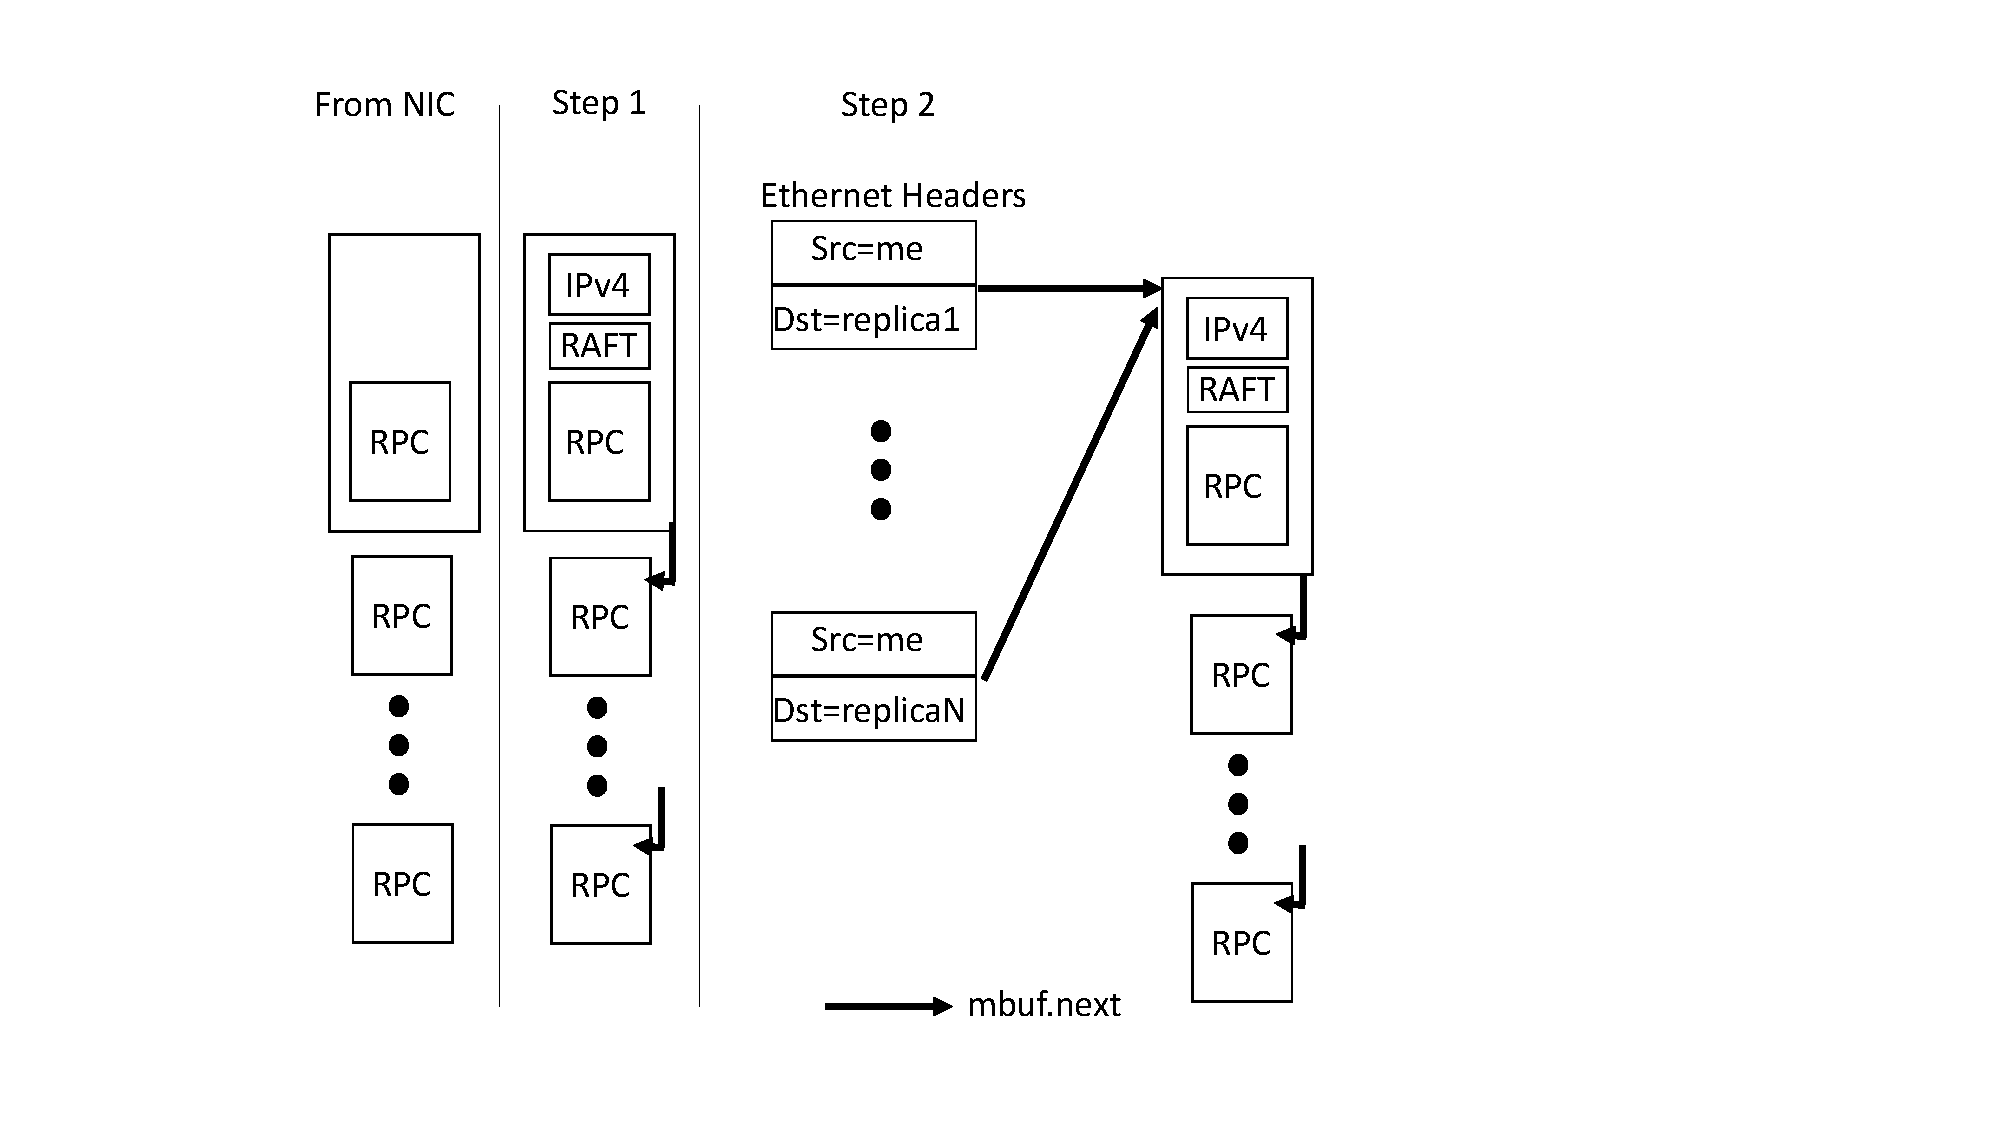
\includegraphics[width=0.9\columnwidth]{figures/chain}
\vspace{-0.15in}
\caption{Zero Copy Batching}
\label{fig:zc_batch}
\end{figure}

\subsection{RPC Call Execution}
\label{sec:exec}
We now describe how RPC calls are executed and results returned to the
client. There are two important aspects of RPC call execution in Cyclone -
steering and at most once semantics.

An RPC call via Cyclone must traverse a specific RAFT core (and associated
consensus protocol instance) and specific application core. These details are
provided by the user when making the RPC call to the Cyclone client side
library. The user therefore is aware of the number of execution cores and RAFT
instances and given complete control of \emph{RPC call steering}. For most
applications we envisage a simple modulo hashing scheme should suffice for load
balancing, something that we plan to later automate in Cyclone.

Cyclone provides at most once semantics. It supports a large but fixed (at
startup time) number of clients. Each RPC call from a client bears the client
number and a sequence number. \emph{Each execution core independently enforces
  that accepted RPC calls from the same client bear increasing sequence
  numbers}. This is done by storing the last executed sequence number for every
client in a per-core durable data structure as part of the crash consistent
transaction wrapping the execution of the RPC call. Even in the presence of
fail-overs, this durable memory of sequence numbers seen from a client ensures
at most once semantics. In addition to guarding against repeated execution of
the same call, Cyclone also remembers the \emph{result} of the last executed RPC
call from every client. This is done to assist clients - particularly stateless
clients. Cyclone allows the client to query the last seen sequence number and
result for that RPC call from any application core on the quorum of servers.

\section{A Durable Replicated Hash Table}
\label{sec:example}
We now demonstrate how Cyclone can be used in practice by putting together an
example of a linearizable hash table - a useful and common data structure.
The baseline is a durable hash table written in NVML that runs on a
single machine in client-server mode. The server side maintains the durable
open-addressed hash table and services client RPC calls to insert and delete
key-value pairs and lookup keys.

A durable hash table is simple to derive from a volatile hash table and readily
available in NVML as an example~\cite{nvml_hash}. To use that (non
client-server) example with Cyclone we added a simple RPC call format, manually
marshalled and demarshalled the few arguments to the RPC call in an RPC call
handler - a few tens of lines of code. Finally, we added a simple client driver
program (a few tens of additional lines of code).

In order to use the hash table with Cyclone, we simply need to to declare the
RPC call handler as the point of entry to Cyclone at the server end.  The client
end issues RPC calls via Cyclone's client side library. Crucially neither side
involves fault awareness or fault recovery code - a key goal for Cyclone.

There are two interesting challenges in scaling the performance and improving
the utility of the linearizable and durable hash table. The first is to ensure
linearizability while scaling performance by adding RAFT cores and application
cores. The second is to support distributed transactions - that manipulate a set
of key-value pairs atomically in the face of failure.

\subsection{Scaling}
Scaling the performance of the hash table by using multiple RAFT cores and
application cores presents determinism related challenges. Two RPC calls being
steered through different RAFT cores can end up executing in different orders on
different replicas even if steered to the same application core. At the same time,
two RPC calls steered through the same RAFT core but dispatched to different
application cores can end up completing in different orders on different replicas.

Our solution to this problem in Cyclone is to observe that replicas of the hash
table require \emph{per-key determinism} and not determinism across \emph{all}
operations. We therefore steer operations to a particular key to the same RAFT
core and the same application core (using a hash on the key).  The actual
configuration of the hash table therefore can be different across different
replicas - for example due to the insertion of two keys mapping to the same hash
bucket completing in different orders across different replicas. However, since
the results of insert, delete and lookup operations for a key depend only on
previous operations to the same key the replicas provide identical results for
committed operations. \emph{In other words, we exploit the fact that operations to
different keys in a map are commutative.}

The RPC call steering mechanism described above leaves the programmer free to
use any synchronization mechanism they wish between concurrent accesses from the
application cores to the data structure, since the ordering between accesses
from different cores is allowed to be non-deterministic. For our open addressed
hash table we chose the simple scheme of a per-bucket lock.

\subsection{Distributed Transactions}
A useful primitive for many distributed systems is the ability to run
distributed transactions - an atomic sequence of conditional updates spanning
multiple groups of replicas. Distributed transactions have two distinct facets:
atomicity and fault tolerance. Distributed transactions appear atomic with
respect to other atomic transactions and simple updates or reads by virtue of
standard concurrency control techniques. A common technique is strict two phase
locking: acquire all locks, update the locked objects and finally release all
the locks. We believe that NVM application programmers - particularly those
with experience in concurrency should not find it hard to deal with
distributed concurrency. The hard part for most programmers is likely to be the
second aspect: fault tolerance. A distributed transaction spans many machines
and has a large footprint to clean up in the event of failure. Failure handling
is made more complex when considering cascading failures - further failures
while recovering from a failure. Cyclone was designed to allow primitives such
as distributed transctions to be added without the programmer needing to worry
about faults or writing fault recovery code. As an exercise we show how to add
support for distributed transactions to our hash table.

We support distributed transactions in our hash table by allowing the user to
specify a group of insert/delete/lookup operations that must occur
atomically. We use the existing bucket locks to support a simple two phase
locking protocol to implement the transction. A client makes an RPC call to the
server specifying the transaction and the server executes it on the client's
behalf. Execution of the transaction has four distinct phases: acquire locks,
verify values, apply updates and finally release locks.

We guard against faults by executing the the entire transaction on a quorum of
machines via Cyclone. All machines in the quorum execute the transaction, making
calls to other quorums to execute steps in the two phase locking protocol. Since
execution of the RPC call leaves \emph{externally visible side effects} by
virtue of the further RPC calls it makes, we require output
commit~\cite{output_commit}. This is achieved if the execution is guaranteed to
complete once it starts. Hence, for distributed transactions, we turn off
decoupled execution (Section~\ref{sec:decouple}).

Next, we need to ensure that although every machine in the quorum makes all
necessary RPC calls, the call itself is executed only once. This is achieved by
using Cyclone's at most once semantics. All machines in the quorum executing the
transaction use the same client identifier and the same montonically increasing
sequence of RPC call numbers. Finally, we need to deal with the fact that
Cyclone only remembers the last executed RPC call for a client. This means that
if different machines in the quorum move at different speeds, some machines will
not receive a response to the RPC call - they will instead receive an error that
tells them that they are too far behind.

To ensure that the transaction is still guaranteed to complete, we use a
\emph{different} client identifier for each \emph{phase}. Thus, until the
transaction completes and a new one is started the response for any RPC call
continues to be available. Figure~\ref{fig:dist_tx} shows in pseudocode the
server side details of a transaction. Once initiated, the distributed transaction
is guaranteed to complete given availability of a quorum.
%However, if the client
%requires intimation of completion, the final transaction state can be written to
%a distinguished partition as part of the transaction itself.

Distributed transactions built around at most once semantics are not intended
for performance. On the other hand, at most once semantics allows users of
Cyclone to avoid writing explicit fault recovery code as compared to fault
recovery in systems that explicity require such cleanup (~\cite{farm}, pp
59--63). Under the assumption that distributed transactions will be infrequent
compared to single key operations, such simplicity is key to increasing the
adoption of NVM among datacenter operators concerned about availability. 

\begin{figure}
{ \scriptsize
\begin{verbatim}
wait until RPC call is replicated
respond to client saying tx accepted for execution
acquire:
 set client identifier to 1
 for each machine
   Acquire write or read locks on the machine
   If machine reponds RPC sequence too old
     Transaction completed by someone else

update:
 set client identifier to 2
 for each machine
   Update object
   If machine reponds RPC sequence too old
     Transaction completed by someone else
 
release:
 set client identifier to 3
 for each machine
   Update object
   If machine reponds RPC sequence too old
     Transaction completed by someone else
\end{verbatim}
}
\vspace{-0.22in}
\caption{Distributed Transactions}
\label{fig:dist_tx}
\end{figure}

\section{Evaluation}
We evaluate Cyclone on a 12 node cluster connected via a 10 GigE switch. Three
of the machines are equipped with 1.6TB Intel DC P3600 SSDs and 4*10 GigE
ports. The remaining nine machines do not have SSDs and have only one 10 GigE
port, serving as clients for most of the experiments. As with other
work~\cite{faast}, we use DRAM on the machines to proxy for NVDIMMs where
necessary - the persistent memory needed never exceeds 64 MB regardless of the
size of the key value store or second level log on flash. We divide the
evaluation into three parts. First, we evaluate Cyclone's performance with a
single level log as a pure software packet switch. Next, we evaluate performance
when adding a second level of log on flash. Finally, we evaluate performance
when integrated with Rocksdb as an alternative to Rocksdb's write ahead
log. Unless otherwise mentioned, we use a 60 byte header followed by a payload
for experiments. We log both the header and payload. In all cases the server
echoes the received entry (header and payload) back to the client. We fix the
number of application threads at 32 using at most 8 threads for running RAFT
instances.

Cyclone is built on top of DPDK to apply software packet switching techniques to
the log replication problem. We therefore begin by systematically evaluating
optimizations applied in Cyclone to replicate the top level log in
Figure~\ref{fig:network_opts} - with no payload. The y-axis reports latency seen
at the client (which means two network round trips with replication). Using
TCP/IP to replicate a RAFT log tops out at around 30K entries/s. Applying
optimizations improves performance by a large enough amount that we use a log
scale on the x-axis. Switching to DPDK (the line marked +DPDK) improves the
throughput by an order of magnitude to around 50K entries/s. Using batching
(line marked +batching) improves the performance further bringing us close to a
million entries/s. Scaling horizontally to 8 physical logs (+8 phy logs)
improves performance to close to 2M entries/s. Finally using all 4 ports on the
machine to replicate entries improves performance considerably to 6M
entries/s. In all performance improves by 200X over the TCP/IP single log
baseline. Cyclone also considerably improves the latency for replication, from
close to 100us with TCP/IP to around 30us at peak throughput.

\begin{figure}
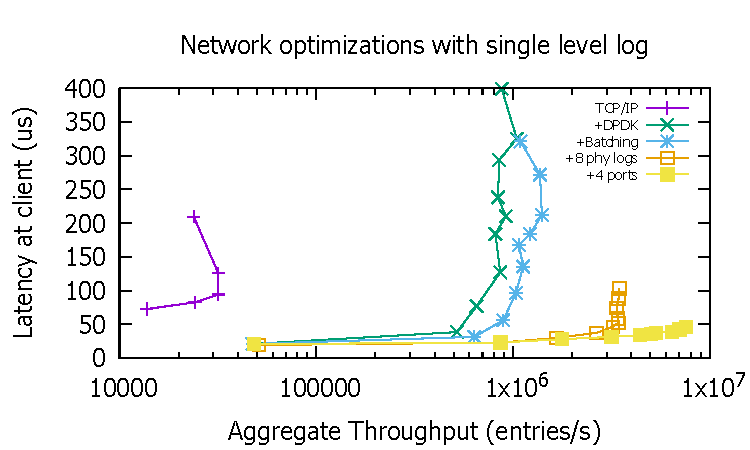
\includegraphics[scale=0.6]{results2/network_opts.pdf}
\caption{Network optimizations for top level log}
\label{fig:network_opts}
\end{figure}

There are two factors that can have significant impact on Cyclone's
performance. First, the number of replicas dictates the outgoing message rate
from the leader replica and therefore increasing the replication factor can
decrease Cyclone's performance. Figure~\ref{fig:replicas} shows the impact of
varying replica count. Using only a single replica cuts out a network round trip
and shows the best unloaded latency (10 us) and peak throughput (near 10M
entries/s). Adding replicas decreases the peak throughput down to around 2M
entries/s. We note that a number of previous pieces of work~\cite{faast, farm}
use three replicas and therefore we focus on three replicas for the replicated
cases we consider below. The second factor that dictates Cyclone's performance
is the size of the log entry being replicated. Figure~\ref{fig:payload} shows
the effect of increasing the payload size from zero to 512 bytes. Peak
throughput drops from 6M entries/s to approximately 2M entries/s. At this
replication rate, the leader replica needs to transmit data at approximately 30
Gbit/s. Coupled with the cost of network headers all four 10 GigE ports are now
saturated and therefore Cyclone hits the network line rate bottleneck at this
point.

\begin{figure}
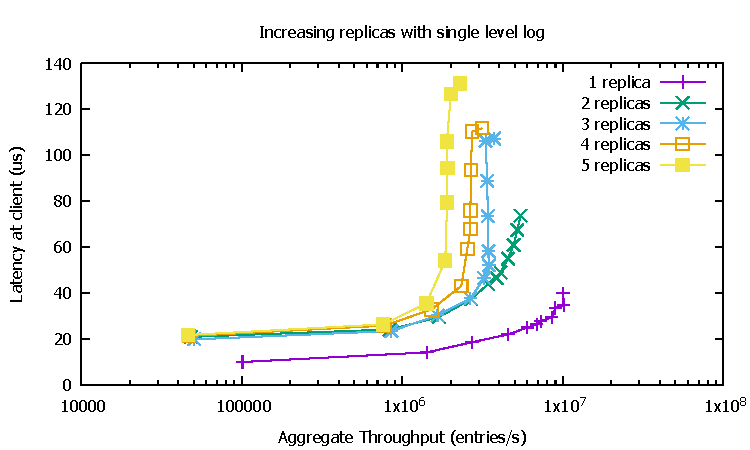
\includegraphics[scale=0.6]{results2/replicas.pdf}
\caption{Impact of replica count}
\label{fig:replicas}
\end{figure}

\begin{figure}
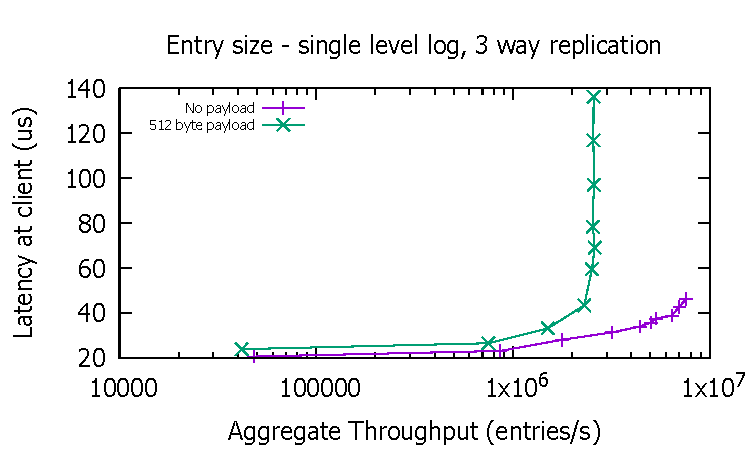
\includegraphics[scale=0.6]{results2/512.pdf}
\caption{Impact of payload size}
\label{fig:payload}
\end{figure}

We now turn our attention from the network component of Cyclone to the storage
one by adding the second level flashlog. We evaluate the impact of adding
storage to our hitherto pure packet switching scenario in
Figure~\ref{fig:flashlog}. Batching entries from the top level NVDIMM log to the
second level flashlog is clearly beneficial as adding flash storage at the
second level has almost no impact on peak performance in Cyclone for small
entries. The situation however changes for larger
entries. Figure~\ref{fig:flashlog_512} shows that using a 512 byte payload has a
significant impact on peak throughput - it drops to approximately 350K
ops/sec. This corresponds to around 50K 4KB IOPS to the SSD to write out the
flashlog pages. The peak for the drive is 160K IOPS using a queue depth
(concurrency) of 128. With 32 application threads we expect a lower peak
throughput around 40K IOPS explaining our bottleneck at 50K IOPS.  It is
possible to tune our observed performance further by aligning the flush boundary
to increase the number of outstanding requests - we do not do so in this paper,
keeping Cyclone agnostic to the exact size of entry being replicated. A final
point about Figure~\ref{fig:flashlog_512} is that once we are past the storage
bottleneck the latency spike is dramatic and large enough to trigger Cyclone's
failure detector and repeated retries from the clients. There are - therefore -
no points on the ``knee'' of the curve as in the pure packet switched one level
log case.

\begin{figure}
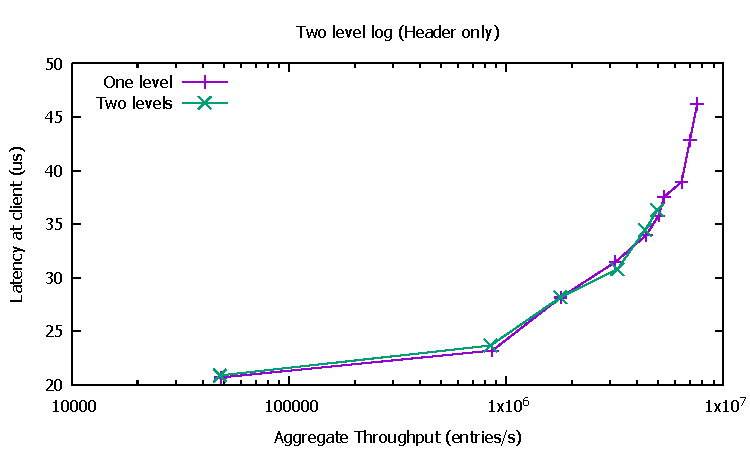
\includegraphics[scale=0.6]{results2/flashlog.pdf}
\caption{Impact of adding second level log}
\label{fig:flashlog}
\end{figure}

\begin{figure}
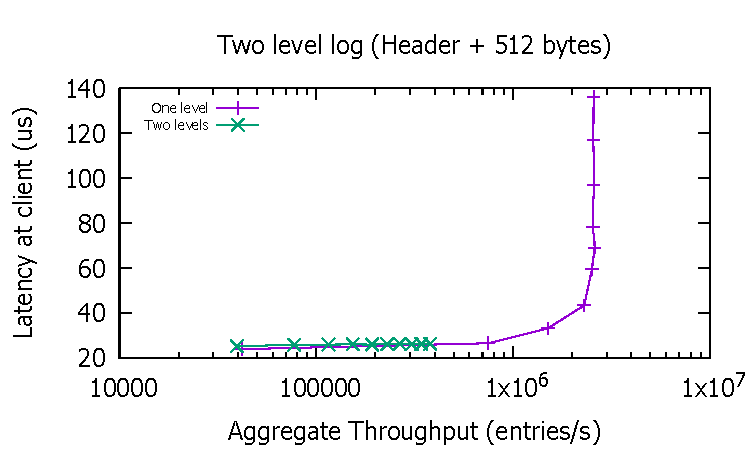
\includegraphics[scale=0.6]{results2/flashlog_512.pdf}
\caption{Impact of adding second level log (512 bytes payload)}
\label{fig:flashlog_512}
\end{figure}

The final dimension we evaluate is of ganged operations. The primary purpose of
ganged operations is to avoid the need for distributed transactions to
manipulate what is a single shared memory image and therefore we were most
concerned about unloaded latency given the complexity of synchronizing different
replication quorums as well executing our rendezvous protocol on multiple
cores. We therefore setup an experiment where a single client reflecting the
unloaded case made ganged requests to the replicas. We varied the number of
cores participating in the request from one to the full complement of 32
application cores. Figure~\ref{fig:ganged} shows the results both using a single
level log as well as a two level log. The primary takeaway is that unloaded
latency increases slowly as we increase the number of active cores - to around
40 us from the baseline of 20 us. There are two causes of this. First, there is
a rapid increase from 1 to 8 active cores, the reason being that this
corresponds to an increase in the number of quorums that must be synchronized
on. There is some amount of synchronization involved in the userspace DPDK
driver for access to common resources for accessing the NIC and this affects the
ability to simultaneously issues replication messages on all quorums. The
smaller contribution to increasing latency that continues past the 8 core case
is due to cacheline pingponging when executing the rendevous. Both these sources
of latency drift could be corrected using replication quorums mapped to
dedicated NICs and more scalable rendesvous designs (such as with machine aware
broadcast trees~\cite{broadcast_tree}). However we deemed the complexity of such
optimizations unnecessary. The added latency for most cases is well under the
extra round trip delay, which would the minimum needed for a solution using
distributed transactions via two phase commit.

\begin{figure}
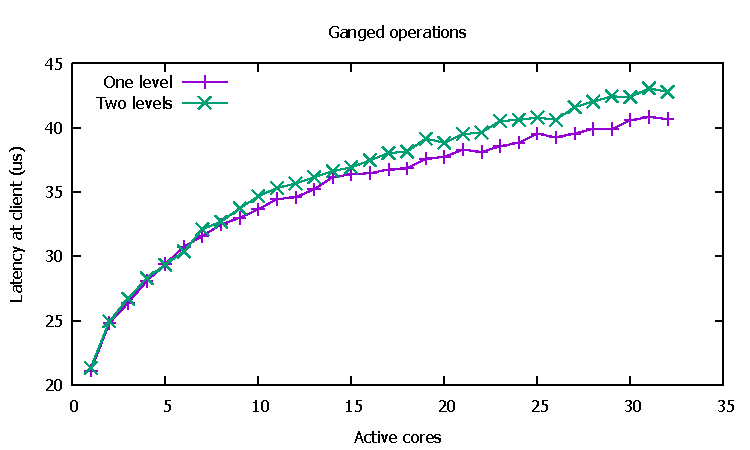
\includegraphics[scale=0.6]{results2/multi.pdf}
\caption{Ganged Operations}
\label{fig:ganged}
\end{figure}

\section{Conclusion}
Cyclone allows developers to add availability to key value maps built on top of
libraries such as NVML and achieve good performance on commodity networking
hardware. A key question is whether Cyclone can be used for other applications
such as filesystems? \emph{We believe that the requirement for scaling across
  multiple replication quorums can be satisfied by applications where the
  scalable commutativity rule~\cite{scalable_commutativity} applies to common
  case primitives.} Although our intitial release of Cyclone will be for key
value style applications, our on-going research is based on the scalable
commutativity hypothesis.
\newcommand\myurl[2]{\url{#1}}
\bibliographystyle{plainnat}
\bibliography{paper}

\end{document}



